%
% dreieck.tex -- slide template
%
% (c) 2021 Prof Dr Andreas Müller, OST Ostschweizer Fachhochschule
%
\bgroup
\begin{frame}[t]
\setlength{\abovedisplayskip}{5pt}
\setlength{\belowdisplayskip}{5pt}
\frametitle{Verallgemeinerte Dreiecksungleichung}
\vspace{-20pt}
\begin{columns}[t,onlytextwidth]
\begin{column}{0.32\textwidth}
\begin{block}{Satz}
\[
|u+v|\le |u|+|v|
\]
Gleichheit wenn lin.~abh.
\end{block}
\begin{block}{Satz}
\[
\biggl|\sum_i u_i\biggr|
\le
\sum_i |u_i|
\]
Gleichheit wenn $u_i = \lambda_i u$
\end{block}
\begin{block}{Satz}
\[
\biggl|\sum_i z_i\biggr|
\le
\sum_i |z_i|
\]
Gleichheit, wenn $z_i=|z_i|c$, $c\in\mathbb{C}$
\end{block}
\end{column}
\begin{column}{0.68\textwidth}
\begin{center}
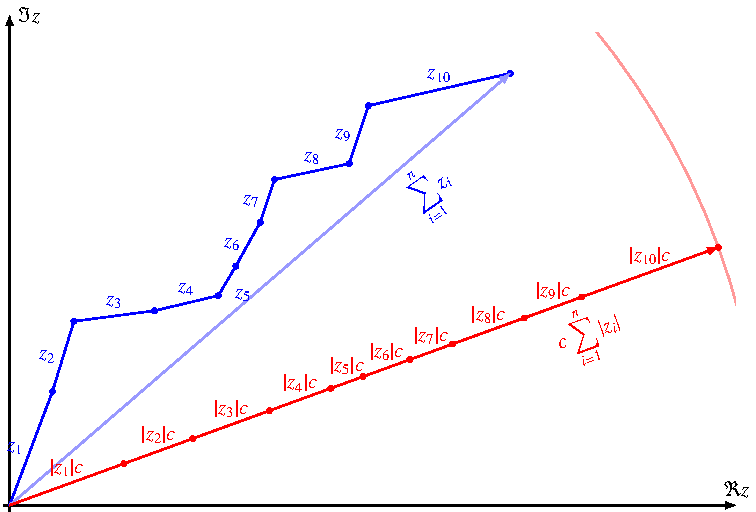
\includegraphics[width=\textwidth]{../../buch/chapters/80-wahrscheinlichkeit/images/dreieck.pdf}
\end{center}
\end{column}
\end{columns}
\end{frame}
\egroup
